\section{Оценка сходимости метода сопряженных градиентов для линейной системы с произвольной симметричной положительно определенной матрицей. Случай $\lambda_1 >> \lambda_2$.}

\subsection{Общий случай}

\begin{theorem*}
	Пусть $A = A^\top$. Тогда для CG справедлива следующая оценка:
	$$\norm[A]{e_k} \le \min_{p_k:p_k(0) = 1} \max_i |p_k(\lambda_i)|\norm[A]{e_0}$$
	Где $p_k$ - многочлен степени $k$, $\lambda_i$ - собственное значение $A$, причем $\lambda_{i} \ge \lambda_{i+1}$
\end{theorem*}

\begin{proof}
	\hphantom{a}\\
	1)\ $\begin{cases}
		x_k = x_0 + y \\
		y \in \mathcal{K}_k(A, r_0)
	\end{cases} \implies x_k = x_0 + q_{k-1}(A)r_0$, где $q_{k-1}$ - полином степени $k-1$. $\implies$ \\
	$\implies r_k = b - Ax_k = b - A(x_0 + q_{k-1}(A)r_0) = \underbrace{(b - Ax_0)}_{\mathclap{r_0}} - Aq_{k-1}(A)r_0 = (I - Aq_{k-1}(A))r_0 = p_k(A)r_0$ \\
	Так как $A$ может быть равна $0$, то, чтобы обнулить ошибку $p_k(0) = 1$. \\
	2)\ $\norm[A]{e_k}^2 = (e_k, Ae_k) = (*)$ \\
	Заметим, что $Ae_k = A(x_*-x_k) = b - Ax_k = r_k \implies (*) = (e_k, r_k) = (*) = (A^{-1}r_k, r_k) = (A^{-1}p_k(A)r_0, p_k(A)r_0)$ \\
	Так как $A$ симметрична и положительно определена, то у нее есть полный ортогональный базис в пространстве собственных векторов $\{v_i\}$, тогда разложим $r_0$ по нему. \\
	$$(A^{-1}p_k(A)r_0, p_k(A)r_0) = \left(A^{-1}p_k(A)\sum^n_{i=1}c_i v_i, p_k(A)\sum^n_{i=1}c_i v_i\right) = \left(\sum^n_{i=1}c_i A^{-1}p_k(A) v_i, \sum^n_{i=1}c_i p_k(A)v_i\right)$$ \\
	Когда на собственный вектор действует полином от матрицы, то он удлиняется в полином от собственного значения раз. \\
	$$\left(\sum^n_{i=1}c_i A^{-1}p_k(A) v_i, \sum^n_{i=1}c_i p_k(A)v_i\right) = \left(\sum^n_{i=1}c_i \frac{p_k(\lambda_i)}{\lambda_i} v_i, \sum^n_{i=1}c_i p_k(\lambda_i)v_i\right) = \sum^n_{i=1}\sum^n_{j=1}c_ic_j \frac{p_k(\lambda_i)p_k(\lambda_i)}{\lambda_i}(v_i, v_j)$$
	Так как базис ортогонален, то $(v_i, v_j) = \delta_{ij}$ \\
	$$\sum^n_{i=1}c_i^2 \frac{p^2_k(\lambda_i)}{\lambda_i} \le \max_i |p_k(\lambda_i)|^2 \sum^n_{i=1}\frac{c_i^2}{\lambda_i} $$ \\
	Осталось понять, чему равно $\sum^n_{i=1}\frac{c_i^2}{\lambda_i}$, давайте представим, что $p_k(\lambda) = 1\ \forall \lambda$ и подставим в наши формулы, выйдет $(A^{-1}r_0, r_0) = \sum^n_{i=1}\frac{c_i^2}{\lambda_i} = (e_0, Ae_0) = \norm[A]{e_0}$, тоесть:
	$$\norm[A]{e_k}^2 \le \max_i |p_k(\lambda_i)|\norm[A]{e_0}$$ \\
	3) Утверждение 2 верно для любого многочлена степени $k$ который равен 1 в нуле, поэтому можно взять минимум.
\end{proof}

Заметим, что:
$$\max_i |p_k(\lambda_i)| \le \max_{\lambda \in [\lambda_n, \lambda_1]} |p_k(\lambda)|$$

Выберем $p_k = \frac{T_k\left(\frac{\lambda_1 + \lambda_n - 2 \lambda}{\lambda_n-\lambda_1}\right)}{T_k\left(\frac{\lambda_1 + \lambda_n}{\lambda_n-\lambda_1}\right)}$, где $T_k$ - многочлен Чебышева.

Тогда воспользуемся оценкой с лекции 14 и получим:
$$p_k(\lambda) \le  2\left(\frac{\sqrt\frac{\lambda_1}{\lambda_n} - 1}{\sqrt\frac{\lambda_1}{\lambda_n} + 1}\right)^{k}$$

$$0 \le 2\left(\frac{\sqrt\frac{\lambda_1}{\lambda_n} - 1}{\sqrt\frac{\lambda_1}{\lambda_n} + 1}\right)^{k} \implies |p_k(\lambda)| \le 2\left(\frac{\sqrt\frac{\lambda_1}{\lambda_n} - 1}{\sqrt\frac{\lambda_1}{\lambda_n} + 1}\right)^{k}$$

Воспользуемся утверждением 2 и получим:
$$\norm[A]{e_k} \le 2\left(\frac{\sqrt\frac{\lambda_1}{\lambda_n} - 1}{\sqrt\frac{\lambda_1}{\lambda_n} + 1}\right)^{k}\norm[A]{e_0}$$

\begin{center}
	
\includegraphics[scale=0.3]{img/q5_2} \\
\end{center}

\subsection{Случай $\lambda_1 >> \lambda_2$}

\begin{proposal}
	Для $A = A^\top > 0$ и любого многочлена $h(\lambda): h(0) = 1$ степени $k$ верно:
	$$\|e_k\|_A \le \max_i |h(\lambda_i)|\|e_0\|_A$$
\end{proposal}
\begin{center}
	(Следует из утверждения 2)
\end{center}

В общем случае мы использовали многочлен вида:
$$t_k(\lambda) = \frac{T_k\left(\frac{\lambda_1 + \lambda_n - 2 \lambda}{\lambda_n-\lambda_1}\right)}{T_k\left(\frac{\lambda_1 + \lambda_n}{\lambda_n-\lambda_1}\right)}$$

Где $T_k$ - многочлен Чебышева. Такой $t_k$ меньше всего отклоняется от 0 на отрезке $[\lambda_n, \lambda_1]$, однако чем больше отрезок тем больше мы отклоняемся. Вообще говоря нас интересует отклонение только в точках $\lambda \in \{\lambda_1, \lambda_2, \dots, \lambda_n\}$. Давайте рассмотрим другой многочлен:
$$p_k(\lambda) = \frac{T_{k-1}\left(\frac{\lambda_2 + \lambda_n - 2 \lambda}{\lambda_n-\lambda_2}\right)}{T_{k-1}\left(\frac{\lambda_2 + \lambda_n}{\lambda_n-\lambda_2}\right)}\left(1-\frac{\lambda}{\lambda_1}\right)$$


\begin{center}
	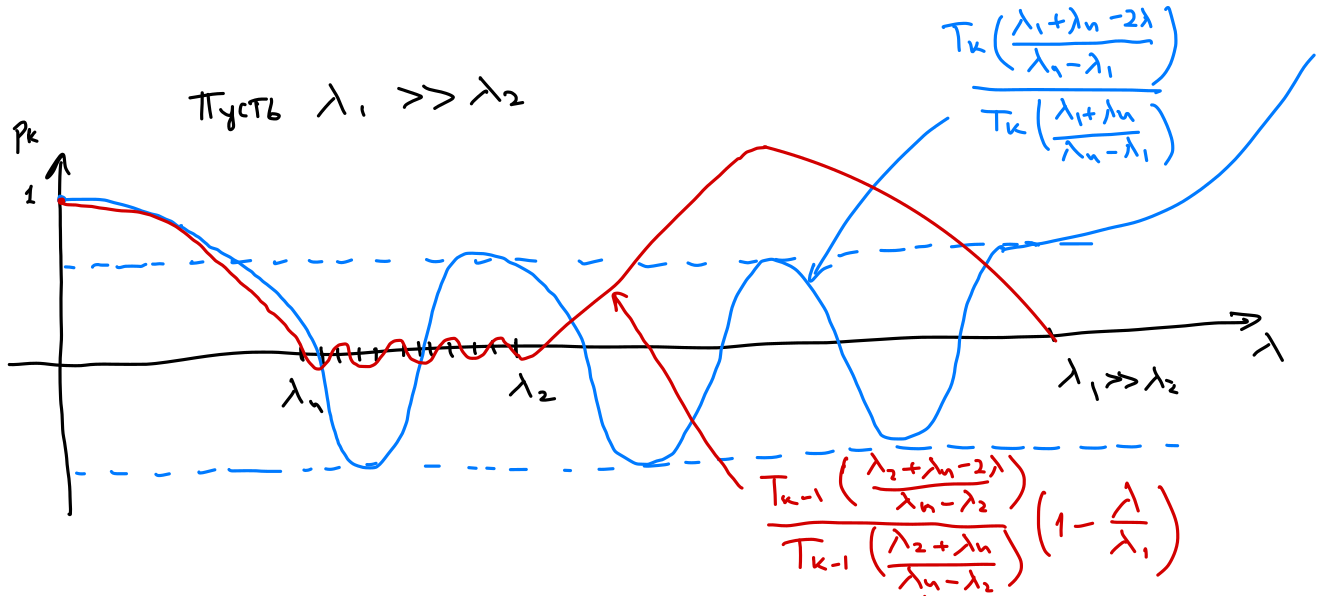
\includegraphics[scale=0.3]{img/q5_1} \\
\end{center}

Тоесть мы уменьшили отрезок, а также пожертвовав степенью многочлена Чебышева, мы добавили множитель который обращается в 0 при $\lambda = \lambda_1$

Нам нужно оценить $\max_i |p_k(\lambda_i)|$, заметим, что:
$$\max_i |p_k(\lambda_i)| \le \max_{\lambda \in [\lambda_{n}, \lambda_2]\cup \{\lambda_1\}}|p_k(\lambda)| = \max_{\lambda \in [\lambda_{n}, \lambda_2]}|p_k(\lambda)|$$

\begin{proposal}
С лекции 14 нам известно:
$$\frac{T_k\left(\frac{a + b - 2 \lambda}{a-b}\right)}{T_k\left(\frac{a + b}{a-b}\right)} \le 2\left(\frac{\sqrt\frac{b}{a} - 1}{\sqrt\frac{b}{a} + 1}\right)^k$$
\end{proposal}

Теперь оценим $p_k$ на множестве $[\lambda_{n}, \lambda_2]$:

\begin{flalign}
	p_k(\lambda) = \frac{T_{k-1}\left(\frac{\lambda_2 + \lambda_n - 2 \lambda}{\lambda_n-\lambda_2}\right)}{T_{k-1}\left(\frac{\lambda_2 + \lambda_n}{\lambda_n-\lambda_2}\right)}\left(1-\frac{\lambda}{\lambda_1}\right) \le 2\left(1-\frac{\lambda}{\lambda_1}\right)\left(\frac{\sqrt\frac{\lambda_2}{\lambda_n} - 1}{\sqrt\frac{\lambda_2}{\lambda_n} + 1}\right)^{k-1} \le 2\left(1-\frac{\lambda_n}{\lambda_1}\right)\left(\frac{\sqrt\frac{\lambda_2}{\lambda_n} - 1}{\sqrt\frac{\lambda_2}{\lambda_n} + 1}\right)^{k-1}
\end{flalign}

Осталось заметить, что $\left| 1-\frac{\lambda_n}{\lambda_1} \right| \le 1$, тогда:
$$p_k(\lambda) \le 2\left(1-\frac{\lambda_n}{\lambda_1}\right)\left(\frac{\sqrt\frac{\lambda_2}{\lambda_n} - 1}{\sqrt\frac{\lambda_2}{\lambda_n} + 1}\right)^{k-1} \le 2\left(\frac{\sqrt\frac{\lambda_2}{\lambda_n} - 1}{\sqrt\frac{\lambda_2}{\lambda_n} + 1}\right)^{k-1}$$

Заметим, что:
$$0\le 2\left(\frac{\sqrt\frac{\lambda_2}{\lambda_n} - 1}{\sqrt\frac{\lambda_2}{\lambda_n} + 1}\right)^{k-1} \implies |p_k(\lambda)| \le 2\left(\frac{\sqrt\frac{\lambda_2}{\lambda_n} - 1}{\sqrt\frac{\lambda_2}{\lambda_n} + 1}\right)^{k-1}$$

Используя первое предложение можно сделать вывод:
$$\|e_k\|_A \le 2\left(\frac{\sqrt\frac{\lambda_2}{\lambda_n} - 1}{\sqrt\frac{\lambda_2}{\lambda_n} + 1}\right)^{k-1}\|e_0\|_A$$
